\documentclass[8pt]{extarticle}
\usepackage{makeidx}
\usepackage{graphicx}
\usepackage{amsmath}
\usepackage{amssymb}
\usepackage{latexsym}
\renewcommand\refname{Referenze}
\usepackage[utf8x]{inputenc}
\usepackage{titlesec}
\usepackage{bm}
\usepackage{mathtools}
\usepackage[document]{ragged2e}
\titleformat{\section}{\huge\normalfont\bf}{\thesection.\hspace{5pt}}{5pt}{\vspace{1cm}}
\titleformat*{\subsection}{\Large\bfseries}
\usepackage[inner=3cm,outer=3cm]{geometry}

\makeindex

\begin{document}
\justify
\printindex
\Large{A.a. 2013-2014}
\vspace{10cm}
\begin{center}
\Huge\textbf{Analisi Dati}
\end{center}

\vspace{2cm}
\begin{flushleft}
\textit{Gruppo \textsc{1}} \\
\medskip
Federico \textsc{Massa} \\ 
Marco \textsc{Montella}
\end{flushleft}



\newpage

\begin{abstract}
\justify
 

\end{abstract}
\bigskip

\section{Introduzione} \label{sec:intro}
Effetto cerenkov, consiste nel rilascio di luce visibile o ultravioletta all'interno di un rivelatore quando esso viene attraversato da una
particella la cui velocità è superiore alla velocità della luce nel mezzo.
Viene pertanto rilasciato un cono di luce con vertice nella posizione della particella e apertura angolare funzione della velocità della particella
e dell'indice di rifrazione del mezzo: \\
\begin{equation} \label{eq:cerenkov}
\cos{\theta}=\frac{1}{n \beta}
\end{equation}

Essendo il coseno di $\theta$ una funzione limitata, fissato un indice di rifrazione si avrà rilascio di fotoni solamente per particelle la cui velocità supera una certa soglia critica: \\
\begin{equation}
\beta > \frac{1}{n}
\end{equation}

Nell'esperimento analizzato, un fascio di particelle composto da mesoni $K$ e $\pi$ attraversano un rivelatore Cerenkov. Uno scintillatore può invece rivelare il passaggio dei muoni prodotti dal loro decadimento. Scopo dell'esperimento è quello di analizzare i segnali provenienti dai due rivelatori e misurare: \\
\begin{itemize}
\item La frazione di K contenuta nel fascio.
\item L'indice di rifrazione del gas che compone il rivelatore Cerenkov.
\item La probabilità di non identificare un mesone $K$ e quella di scambiare un $\pi$ per un $K$, una volta definita una regione di identificazione.
\end{itemize}

\section{Apparato sperimentale} \label{sec:apparato}
I rivelatori Cerenkov sono correlati di una superficie otticamente attiva sulla superficie interna (come nel caso di Super-Kamiokande) o su una delle basi, come nel caso dell'esperimenti NA48/62 (vedere se è vero) e nell'apparato considerato nella presente analisi. (CHECK!!!) Il rivelatore Cerenkov
che si prende in considerazione in questa analisi è dotato, sulla base più lontana relativamente al verso delle particelle del fascio, di uno specchio parabolico la cui lunghezza focale è pari alla lunghezza del rivelatore. Sulla base opposta, in corrispondenza del piano focale, si trova un rivelatore a pixel 50x50 di dimensioni 1cmx1cm. Lo specchio parabolico ha la proprietà di "focalizzare" fasci di luce paralleli su un punto del piano focale funzione dell'angolo formato dal fascio con l'asse ottico, sebbene solo quando questo angolo è zero la messa a fuoco risulta priva di aberrazione. Sulla base otticamente sensibile i pixel interessati dall'arrivo di uno o più fotoni formeranno dunque, a causa della simmetria sull'angolo azimutale, di un anello il cui raggio può essere messo in relazione con l'angolo di emissione dei fotoni, e di conseguenza con la velocità della particella. Essendo la velocità delle particelle costituenti il fascio differente, questo meccanismo può essere sfruttato per l'identificazione. \\

L'apparato sperimentale simulato consiste di un rivelatore Cerenkov a gas di indice di rifrazione $n$ ignoto da determinarsi nell'analisi, di lunghezza $1000 \ cm$, pari alla lunghezza focale dello specchio parabolico posto sul fondo del recipiente contenente il gas. Il rivelatore di fotoni Cerenkov posto sul piano focale dello specchio è un quadrato composto da 2500 pixel ciascuno di dimensioni 1cm x 1cm. \\
\subsection{Formazione degli anelli Cerenkov}
Al passaggio di una particella con $\beta > c/n$, si ha nel gas un'emissione di fotoni visibili o ultravioletti ad un angolo $\theta$ con la direzione del fascio per cui vale l'eq. \eqref{eq:cerenkov}. \\

Il fotone raggiunge lo specchio parabolico e viene riflesso producendo, a meno di inefficienze nella riflessione, nella trasmissione nel gas o nella rivelazione, un segnale in uno dei pixel. Essendoci una simmetria sull'angolo azimutale $\phi$, l'insieme di tutti i fotoni che possono essere emessi dalla particella a una distanza $d$ fissata dal vertice dello specchio forma una circonferenza sul piano focale.\\
\'E possibile dimostrare che il raggio di tale circonferenza è indipendente dal punto di emissione $d$, e che pertanto tutti i fotoni emessi dalla particella nel suo percorso all'interno della camera a gas vengono messi a fuoco su una circonferenza il cui raggio dipende solamente dall'angolo Cerenkov e dalle caratteristiche dello specchio parabolico.\\
Chiamando $\theta$ l'angolo Cerenkov, $d$ la distanza di emissione dal vertice della parabola, $f$ la distanza focale, $\delta$ l'angolo formato dalla tangente alla parabola nel punto di riflessione del fotone con un asse parallelo al piano focale e $x0$ la distanza del punto di riflessione dal vertice della parabola, il raggio $R$ dell'anello Cerenkov risulta:
\begin{equation} \label{eq:raggio_theta}
R \ = \ \frac{f+x_0 \cot{\theta}+x_0 \cot{(\theta-2\delta)}-d}{\cot{(\theta-2\delta)}}
\end{equation}
\begin{equation}
x_0 \ = \frac{f}{2} \Bigg[-\cot{\theta}+\sqrt{\cot{\theta}^2+\frac{d}{f}}\ \Bigg] \ \ \ \ \ \ \ \tan{\delta}=\frac{2x_0}{f}
\end{equation}
La relazione \ref{eq:raggio_theta} è stata plottata in ROOT ad angolo fissato. Nella figura [FIGURA] è mostrato l'andamento del raggio con la distanza di emissione.\\
La non costanza del raggio in funzione di d è dovuta al fatto che uno specchio o una lente parabolica è in grado di mettere a fuoco solamente raggi paralleli all'asse ottico. L'aberrazione sulle immagini provenienti da sorgenti fuori asse è nota come \textit{coma}.
Ad ogni modo lo scarto relativo tra gli estremi di variabilità del raggio è dell'ordine di $10^{-4}$, ed è all'incertezza derivante dalla discretizzazione delle posizioni introdotta dai pixel.\\
Le figure [figure 2 e 3] mostrano invece l'andamento del raggio in funzione contemporaneamente di $\theta$ e $d$. Tale andamento si mostra in ottima approssimazione lineare con l'angolo secondo un coefficiente di proporzionalità pari alla lunghezza focale. Nella figura [FIGURA!!!] è mostrato l'andamento con $\theta$ e $d$ della quantità: $R(\theta,d)-f\theta$.

\subsection{Segnale nello scintillatore}
Ad una distanza di 9000 cm dallo specchio parabolico del rivelatore Cerenkov è posto uno scintillatore dalla forma di corona circolare, con $R_{min}=10\ cm$ e $R_{MAX}=100\ cm$, nel quale vengono rivelati i muoni provenienti da eventuali decadimenti delle particelle del fascio.
L'energia di quest'ultimo, unitamente alle dimensioni dell'apparato, fa si tuttavia che i muoni del canale $\pi^+ \ \rightarrow \ \mu^+ \nu_\mu$ non siano rivelati nello scintillatore, passando sempre a una distanza dall'asse del fascio $r<R_{min}$. \\
Infatti, noto l'angolo $\alpha$ con cui il muone viene emesso nel sistema di riferimento a riposo del pione, risulta per l'angolo $\alpha'$ nel sistema del laboratorio:
\begin{equation}
\tan{\alpha}=\frac{p_T}{p_L}
\end{equation}
\begin{equation}
\tan{\alpha'}=\frac{p_T}{p_L'}=\frac{p\sin{\alpha}}{\gamma_{\pi}\big[p\cos{\alpha}+\beta_{\pi} (p^2+m_mu^2)^{1/2}\big]}
\end{equation}
\\
L'andamento della funzione $\alpha'(\alpha)$ è mostrato in [FIGURA], e presenta un punto  di massimo per $	\alpha=105.523°$ $\rightarrow$ $\alpha'=0.0184°$.\\
Un $\pi$ che decadesse all'interno del Cerenkov dopo aver prodotto segnale in esso produrrebbe pertanto un muone che giungerebbe allo scintillatore con una distanza dall'asse di al massimo $r=10000\ cm \cdot \theta (rad) \simeq 3.2 cm$.\\
\\
Gli eventi di $\pi$ saranno dunque caratterizzati dall'assenza di hits nello scintillatore. La proposizione inversa non è invece vera: essendo $\gamma_K c \tau_K \ \sim 900 \ m$, solo una frazione dei K decadrà nei 100 m coperti dall'apparato. Si considera inoltre che il branching ratio del canale di decadimento $K^+ \rightarrow \mu^+\nu_mu$ a cui è sensibile lo scintillatore è $BR_{\mu 2}=63.5\%$, e anche di questi decadimenti una frazione risulterà in muoni che attraversano il foro dello scintillatore, non producendo ugualmente segnale.
\\
\section{Metodo}
Evento per evento sono forniti il numero di hit (0 o 1) registrati nello scintillatore, il numero di pixel della superficie sensibile del rivelatore Cerenkov interessati dall'arrivo di uno o più fotoni e l'identificativo di questi ultimi secondo uno schema a griglia.\\
\subsection{Ricostruzione del raggio dell'anello Cerenkov}
La ricostruzione evento per evento del raggio dell'anello Cerenkov è stata portata a termine seguendo il metodo dei minimi quadrati adattato ad una funzione di fit circolare. La procedura, spiegata in [REFERENZA DAL DOCUMENTO DI GIUDICI], consiste nell'identificazione di centro e raggio della circonferenza minimizzando la quantità:
\begin{equation}
S=\sum_i g(u_i, v_i, R)^2 \ = \ \sum_i \Big[ (u_i-u_c)^2+(v_i-v_c)^2 - R^2 \Big]
\end{equation}
\\
Dove $u_i, v_i$ rappresentano le coordinate di ciascun pixel di interesse in un sistema cartesiano centrato di volta in volta nella media dei pixel attivi $( \ u_i=x_i-\sum_j x_j /N\ )$. La minimizzazione viene effettuata rispetto ai parametri del fit $u_c, v_c, R$ coordinate del centro del cerchio e raggio di quest'ultimo.\\
I risultati dei fit ottenuti nei $50\ 000$ eventi sono mostrato nella figura sottostante. [FIGURA ISTOGRAMMI]
A causa della risoluzione sperimentale, ad ogni particella non corrisponde un raggio ben definito, ma una distribuzione la cui deviazione standard potrà essere utilizzata per stimare l'errore.

\subsection{Frazione di K nel fascio}
Nell'assunto che i raggi degli anelli generati dal passaggio delle due particelle siano distribuiti secondo una Normale con media $\mu_{K,\pi}=\theta_{K,\pi}f$ e varianza determinata dalla risoluzione sperimentale, l'istogramma dei raggi negli eventi disponibili è stato fittato con la somma di due distribuzioni gaussiane.\\
\\
A partire dai parametri ottenuti ottenuti dal fit il numero di mesoni $K$ e $\pi$ sono stati ottenute integrando separatamente le due distribuzioni appena determinate.\\
\subsubsection{Incertezza su $f_K$}
L'incertezza sulla frazione di K nel fascio è stata calcolata con il metodo degli pseudo esperimenti. Il contenuto di ciascun bin dell'istogramma è distribuito secondo una Binomiale con probabilità di successo della prova stimata in $\hat{\mu}_i = N_{i}/N$, con $N_i$ contenuto dell'i-esimo bin e N numero totale di eventi. A partire da tale distribuzione il contenuto dei bin è stato fatto variare casualmente, ottenendo così una serie di pseudo distribuzioni di raggi Cerenkov, a loro volta fittate ciascuna con una somma di due gaussiane.\\
La frazione dei mesoni $K$ è stata ottenuta come valor medio della distribuzione di $f_K$ nei vari pseudo esperimenti, e si è utilizzata la deviazione standard di tale distribuzione come incertezza sul valore sperimentale di $f_K$

\subsection{Misura dell'indice di rifrazione}
La relazione (\eqref{eq:raggio_theta}) può essere riformulata in funzione di massa della particella e indice di rifrazione sfruttando l'uguaglianza (\eqref{eq:cerenkov}) e il fatto che $\beta^2=(1+\gamma^{-2})=(1+\frac{m^2}{E^2})$. In questo modo si ottiene una relazione che invertita permette di misurare l'indice di rifrazione in funzione del raggio misurato. Essendo quest'ultimo noto con una data incertezza, anche l'indice di rifrazione avrà una sua incertezza. Quest'ultima è stata calcolata misurando il valore dell'indice di rifrazione al variare del raggio secondo la distribuzione misurata. L'indice di rifrazione può essere calcolato sia a partire dai dati relativi ai mesoni $K$, sia da quelli relativi ai mesoni $\pi$. Essendo il mezzo attraversato dalle particelle lo stesso, si è controllato, per verifica, che i risultati ottenuti nei due modi fossero compatibili.

\subsection{Intervallo di confidenza per l'identificazione dei K}
A causa dell'elevata energia del fascio rispetto alle masse delle due specie di particelle, i $\beta$ dei $\pi$ e dei $K$ sono molto simili, ragion per cui ci si attende un intervallo di raggi per cui esiste una probabilità non trascurabile, date le rispettive distribuzioni, di avere un evento sia di $\pi$ che di $K$.\\
Volendo assicurare una procedura per l'identificazione dei K del fascio con un certa confidenza a discrezione dello sperimentatore, è necessario definire in relazione a tale livello di confidenza un intervallo di valori per il raggio dell'anello rivelato nella camera a gas.\\
La finalità primaria della determinazione dell'intervallo di confidenza risiede nella minimizzazione della probabilità che un evento identificato come $K$ sia in realtà un $\pi$, massimizzando in tal modo la purezza del fascio di K.\\
Un taglio severo sul raggio dell'anello Cerenkov porta tuttavia anche all'aumento della frazione di legittimi eventi di $K$ scartati in quanto fuori dall'intervallo di confidenza. A seconda delle finalità dell'esperimento e dalle esigenze sperimentali si può scegliere un intervallo molto severo che permetta di usare l'apparato come un trigger "purificando" il fascio a scapito della luminosità, o alternativamente un intervallo più lasco favorendo il numero di eventi totali sulla purezza del fascio.
\subsubsection{Probabilità di identificare un $\pi$ come un K}
L'estremo inferiore dell'intervallo di confidenza è posto a $\bar{R_K}-d\sigma_K$
\subsubsection{Probabilità di non identificare un K}

\section{Risultati}

\subsection{Indice di rifrazione}
Le fig. \ref{fig:indiceK} e \ref{fig:indicePI} riportano le distribuzioni dell'indice di rifrazione ottenute tenendo conto delle distribuzioni dei raggi. Risulta: \\

\begin{figure}
\begin{center}
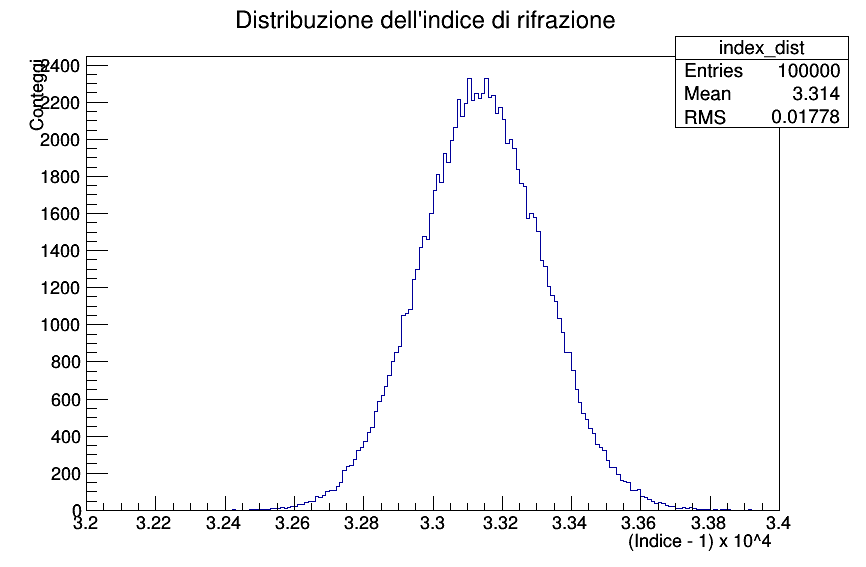
\includegraphics[scale=0.4]{indiceK_definitivo}
\caption{Distribuzione dell'indice di rifrazione ottenuto utilizzando la distribuzione dei raggi associati al passaggio di un mesone $K$.}
\label{fig:indiceK}
\end{center}
\end{figure}

\begin{figure}
\begin{center}
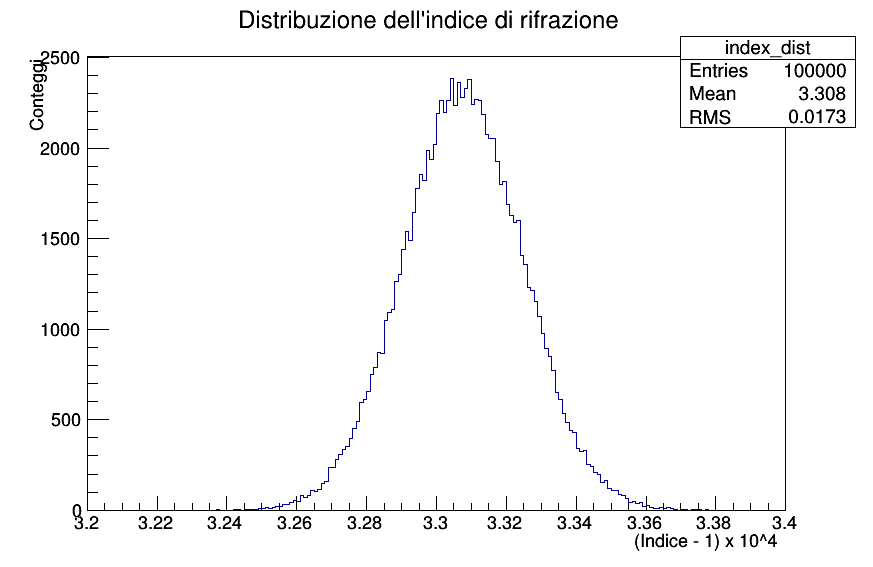
\includegraphics[scale=0.4]{indicePI_definitivo}
\caption{Distribuzione dell'indice di rifrazione ottenuto utilizzando la distribuzione dei raggi associati al passaggio di un mesone $\pi$.}
\label{fig:indicePI}
\end{center}
\end{figure}

I risultati sono quindi perfettamente compatibili: \\
\begin{equation}
n_K -1 = (3.31 \pm 0.02) \cdot 10^{-4}
\nonumber
\end{equation}

\begin{equation}
n_{\pi} -1 = (3.31 \pm 0.02) \cdot 10^{-4}
\nonumber
\end{equation}

\section{Conclusioni}
Cosa si può cambiare nell'apparato per migliorare l'identificazione? Indice di rifrazione?

%\input{bibcompton.bib}


\end{document}
